\section{Evaluation of Fides Resilience}
\label{sec:fides-resilience}

To evaluate the resilience of Fides in different scenarios, we need to find the optimal configuration for the following parameters in Fides: interaction evaluation strategy (Section~\ref{sec:interaction-evaluation-strategies}), threat intelligence aggregation function (Section~\ref{sec:network-intelligence-aggregation}) and initial reputation (Section~\ref{subsubsec:computing-reputation}). Each combination of parameters is evaluated in its capacity to correctly classify targets in \textit{any} network topology.\footnote{Distribution of correct/uncertain/incorrect/malicious peers in the network.}

In this section, we are focusing on finding the best possible combination of parameters for the worst possible scenario. In other words, we want to identify a setup, where the Fides can guarantee that it is eventually going to provide the correct data and will classify the targets correctly even though the malicious actor controls most of the network.

We shows two specific scenarios - one with no pre-trusted peers and one where there are 25\% of peers part of some pre-trusted organization. Because even the scenario with only 25\% peers shows, that in some case is Fides able to defend itself against the rest of the network, we do not show scenarios with more pre-trusted peers, but we include them in the appendix (Figure~\ref{fig:performance-all-setups-50-pretrusted}).

\subsection{Scenario With No Pre-Trusted Peers}
\label{subsec:scenario-with-0-pretrusted-peers}

In this scenario, there are no pre-trusted peers nor organizations and Fides needs to determine trust in each peer by itself.
We simulated environments starting with the 75\% of confident correct peers~(behavior from Section~\ref{subsubsec:confident-correct-peer}) up to 75\% malicious peers~(behavior from Section~\ref{subsubsec:malicious-peer}) and used all possible setups.

\cleartoleftpage % check if this appears on the left side 
\subsubsection{Target Detection Performance}

The target detection performance $tdp$ (Section~\ref{subsec:target-detection-performance-metric}) is the most important metric because it evaluates how good is Fides in the target classification - if the Fides is able to correctly come up to a conclusion that \textit{evil.com} is malicious target and \textit{google.com} is the benign.

Figure~\ref{fig:25-target-detection} visualizes the target detection performance on three different graphs where each of the graphs is a single interaction evaluation strategy.
Each graph then displays dots with different colors. Each color a single threat intelligence aggregation method in combination with different initial reputation value.
A single dot in the graph is the value of $tdp$ and in a case when the $tdp \geq 1$, it means that Fides made on average the wrong decision about the targets and classified them with the wrong label.
In other words, if $tdp \geq 1$, Fides classified benign targets as malicious and the other way around.
We included the \textit{red line} that shows $tdp = 1$ so if a dot is above the \textit{red line}, the Fides made incorrect target classification.
For that reason, we optimize the \textit{dots} to be \textit{below} the \textit{red line} (classifications being correct).

The horizontal axis in each graph measures the environment hardness explained in Section~\ref{subsec:environment-hardness}. It is important to note, that hardness essentially expresses how many peers that can provide correct data are in the simulation. For example, if the hardness is $10$, $100\%$ of peers inside the simulation are providing correct data and behave like confident correct peers.
Thus the higher the value of hardness is, the easier it is for the Fides to do correct classification.

Specifically in Figure~\ref{fig:0-target-detection} we can see that that in the \textit{easy} environment, most of the \textit{dots} are below the red line until the hardness gets close to $3$.
The metrics perform more or less the same as they are able to stay bellow the red line until $eh = 3$. In that situation, the best performance and thus the lowest $tdp$ has $ThresholdTIEvaluation$ in combination with $WeighedDistanceToLocalTIEvaluation$ and initial reputation of $0.95$.

Interestingly, the $DistanceBasedTIEvaluation$ in combination with $0$ initial reputation and $AverageConfidenceTIAggregation$ for threat intelligence aggregation, shows the same target classification performance in each environment - $tdp = 0$. This suggests that the method was unable to determine any trust for any of the peers. This is then later confirmed by the Figure~\ref{fig:0-peer-trust}.

% TODO: move the legend to the left
\begin{figure}[hp]
    \centering
    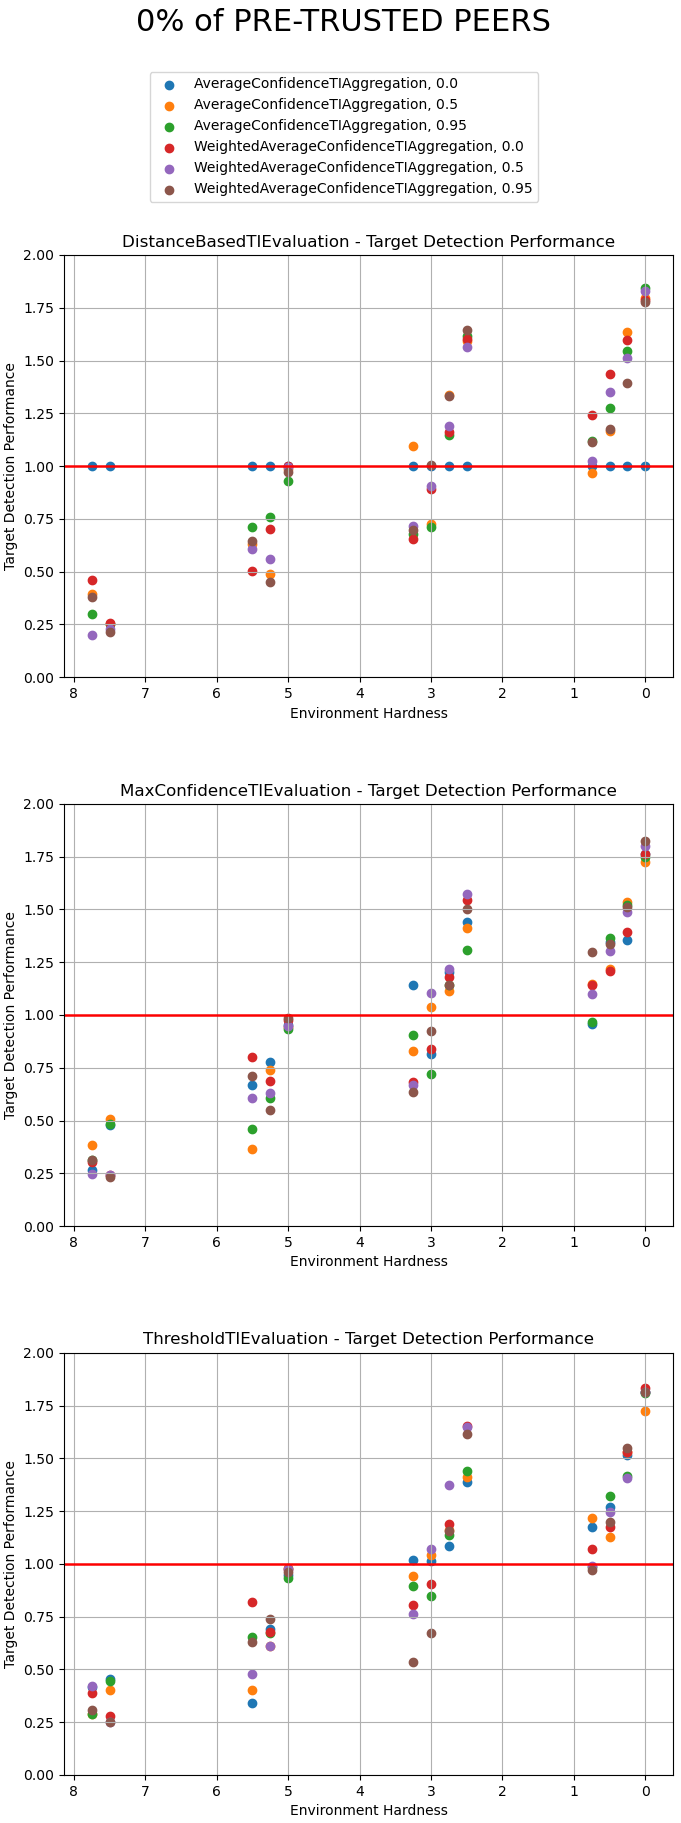
\includegraphics[height=0.9\textheight]{assets/0_target_detection.png}
    \caption{Target detection performance (vertical axis) for three different interaction evaluation strategies in different environments (horizontal axis) with \textbf{no pre-trusted peers}.}
    \label{fig:0-target-detection}
\end{figure}

\cleartoleftpage
\subsubsection{Peers Behavior Detection Performance}
\begin{figure}[hp]
    \centering
    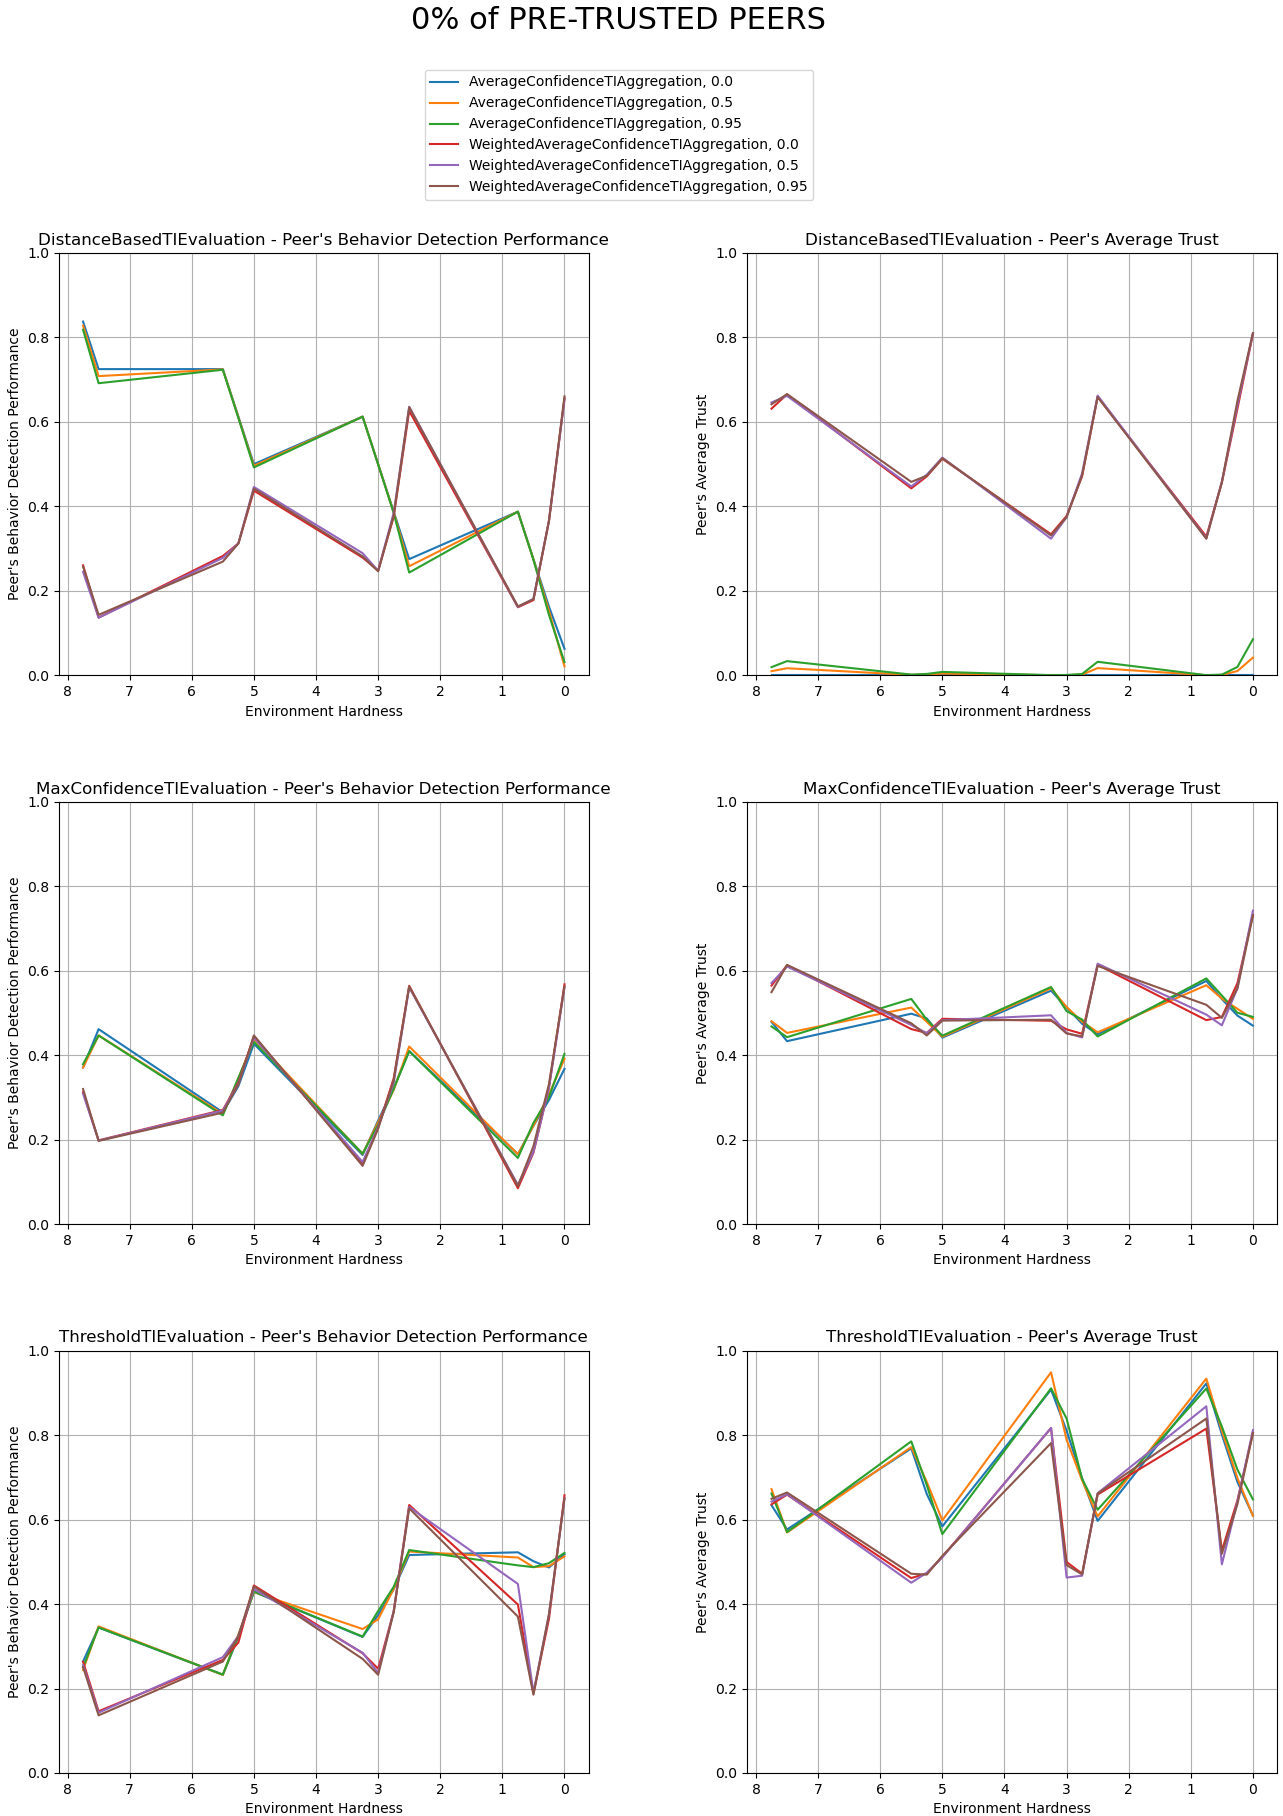
\includegraphics[width=1.0\textwidth]{assets/0_peer_trust.png}
    \caption{Behavior of peer's trust metrics in the different environments for different Fides's setups with \textbf{no pre-trusted peers}. On the left side peer's behavior detection performance, on the right side peer's average trust.}
    \label{fig:0-peer-trust}
\end{figure}

Figure~\ref{fig:0-peer-trust} displays two important metrics which are related to how much does Fides trust the peers in the network. First is peer's behavior detection performance metric $pbdp$ (Section~\ref{subsec:peers-behavior-detection-performance-metric}) and the second is the peer's average trust.

On the left side, one can see the peer's behavior detection performance metric that measures how good was Fides in estimating the peer's behavior. The lower value of $pbdp$ the better because the Fides's service trust for the peer was closer to the real value used in the simulation.

On the right side, we show the peer's average trust metric. That is an average trust of Fides for each peer. We include this metric in order to see how much trust was Fides able to obtain for the peers in the network.
It is important to note, that there is no \textit{correct} or \textit{desired} value of this metric, because for example in the environment where there are all peers confident correct, the peer's average trust should be high, but in the environment with all byzantine peers, this metric should be low because Fides should not trust incorrect and malicious peers.

As suggested in the previous section while measuring target detection performance, the right graph for $DistanceBasedTIEvaluation$ in combination with $AverageConfidenceTIAggregation$ shows, that this setup is unable to determine trust for the peers and has average peer's trust close to $0$. This means that the trust model will almost always aggregate threat intelligence to score $0$ with confidence $0$ making it, in a fact, useless. 

\cleartoleftpage
\subsection{Scenario With 25\% of Pre-Trusted Peers}
\label{subsec:scenario-with-25-pretrusted-peers}

In this scenario, Fides assumes that there are 25\% of pre-trusted peers. We simulated environments starting with the 75\% of confident correct peers~(behavior from Section~\ref{subsubsec:confident-correct-peer}) up to 75\% malicious peers~(behavior from Section~\ref{subsubsec:malicious-peer}) and used all possible setups.

\subsubsection{Target Detection Performance}
\label{subsubsec:target-detection-performance}
% TODO: move the legend to the left
\begin{figure}[hp]
    \centering
    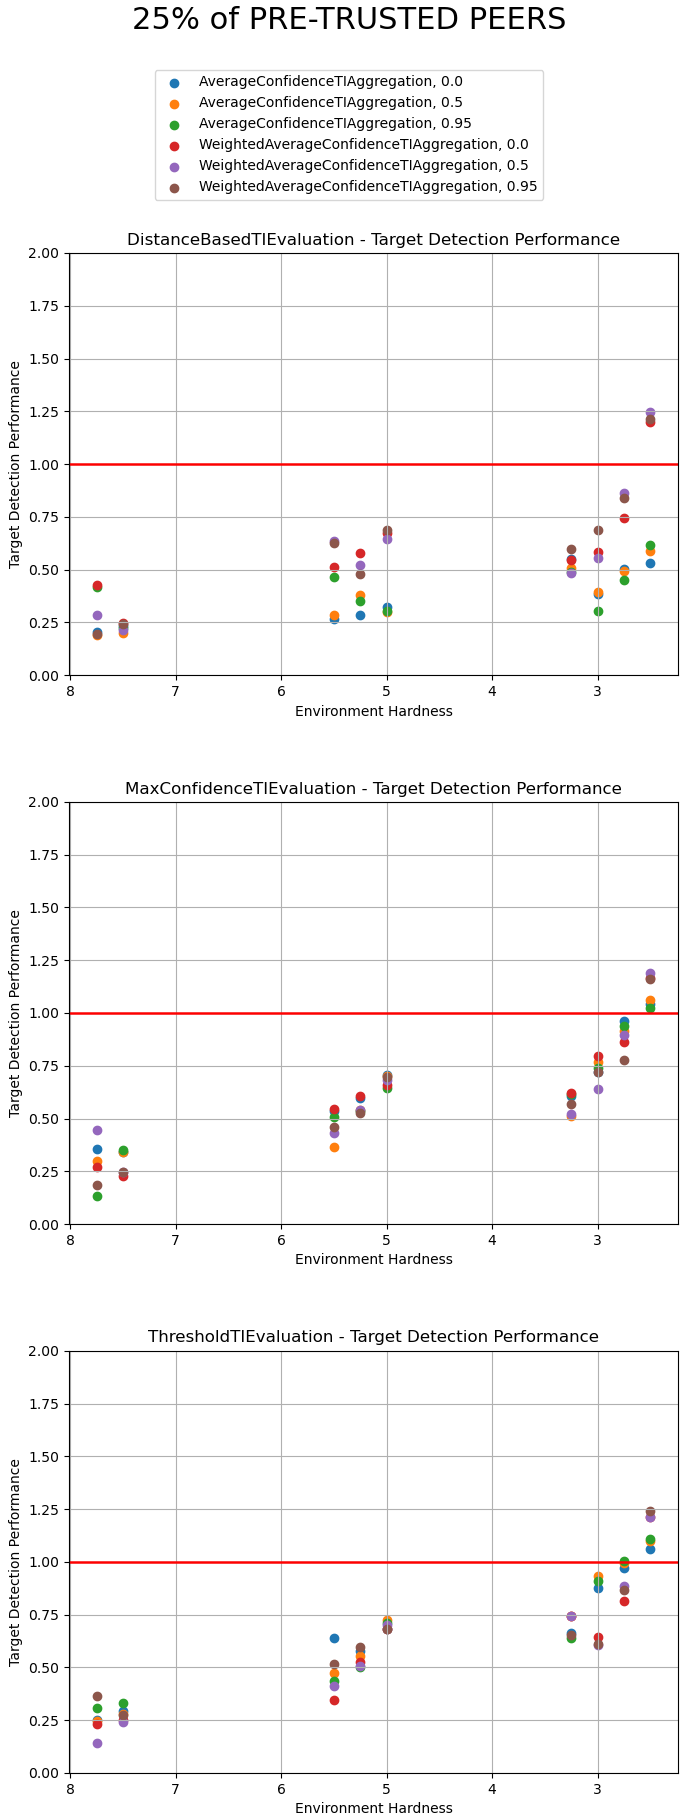
\includegraphics[height=0.9\textheight]{assets/25_target_detection.png}
    \caption{Target detection performance (vertical axis) for three different interaction evaluation strategies in different environments (horizontal axis) with \textbf{25\% pre-trusted peers}.}
    \label{fig:25-target-detection}
\end{figure}

Specifically in Figure~\ref{fig:25-target-detection} one can see that until the environment hardness $eh \geq 3$, all strategies help Fides to classify targets correctly.
That changes after the environment hardness $eh \leq 2.5$ when the $ThresholdTIEvaluation$ as well as $MaxConfidenceTIEvaluation$ misclassify the targets and the $tdp \geq 1$. In that case, all threat intelligence aggregation methods are the same and all of them misclassify the targets no matter what initial reputation is used.
However, the $DistanceBasedTIEvaluation$ strategy in combination with $AverageConfidenceTIAggregation$ method is able to still classify the targets correctly and maintain the $tdp \leq 1$ even under toughest conditions where there are 75\% of adversarial peers in the simulation.

When Fides is used in a similar situation with the threat intelligence aggregation method $WeightedAverageConfidenceTIAggregation$, it misclassified the targets in one simulation when working in the hardest environment.
Thus, this method does not provide a guarantee that Fides will end up with correct classifications for every target.

\cleartoleftpage
\subsubsection{Peers Behavior Detection Performance}

\begin{figure}[hp]
    \centering
    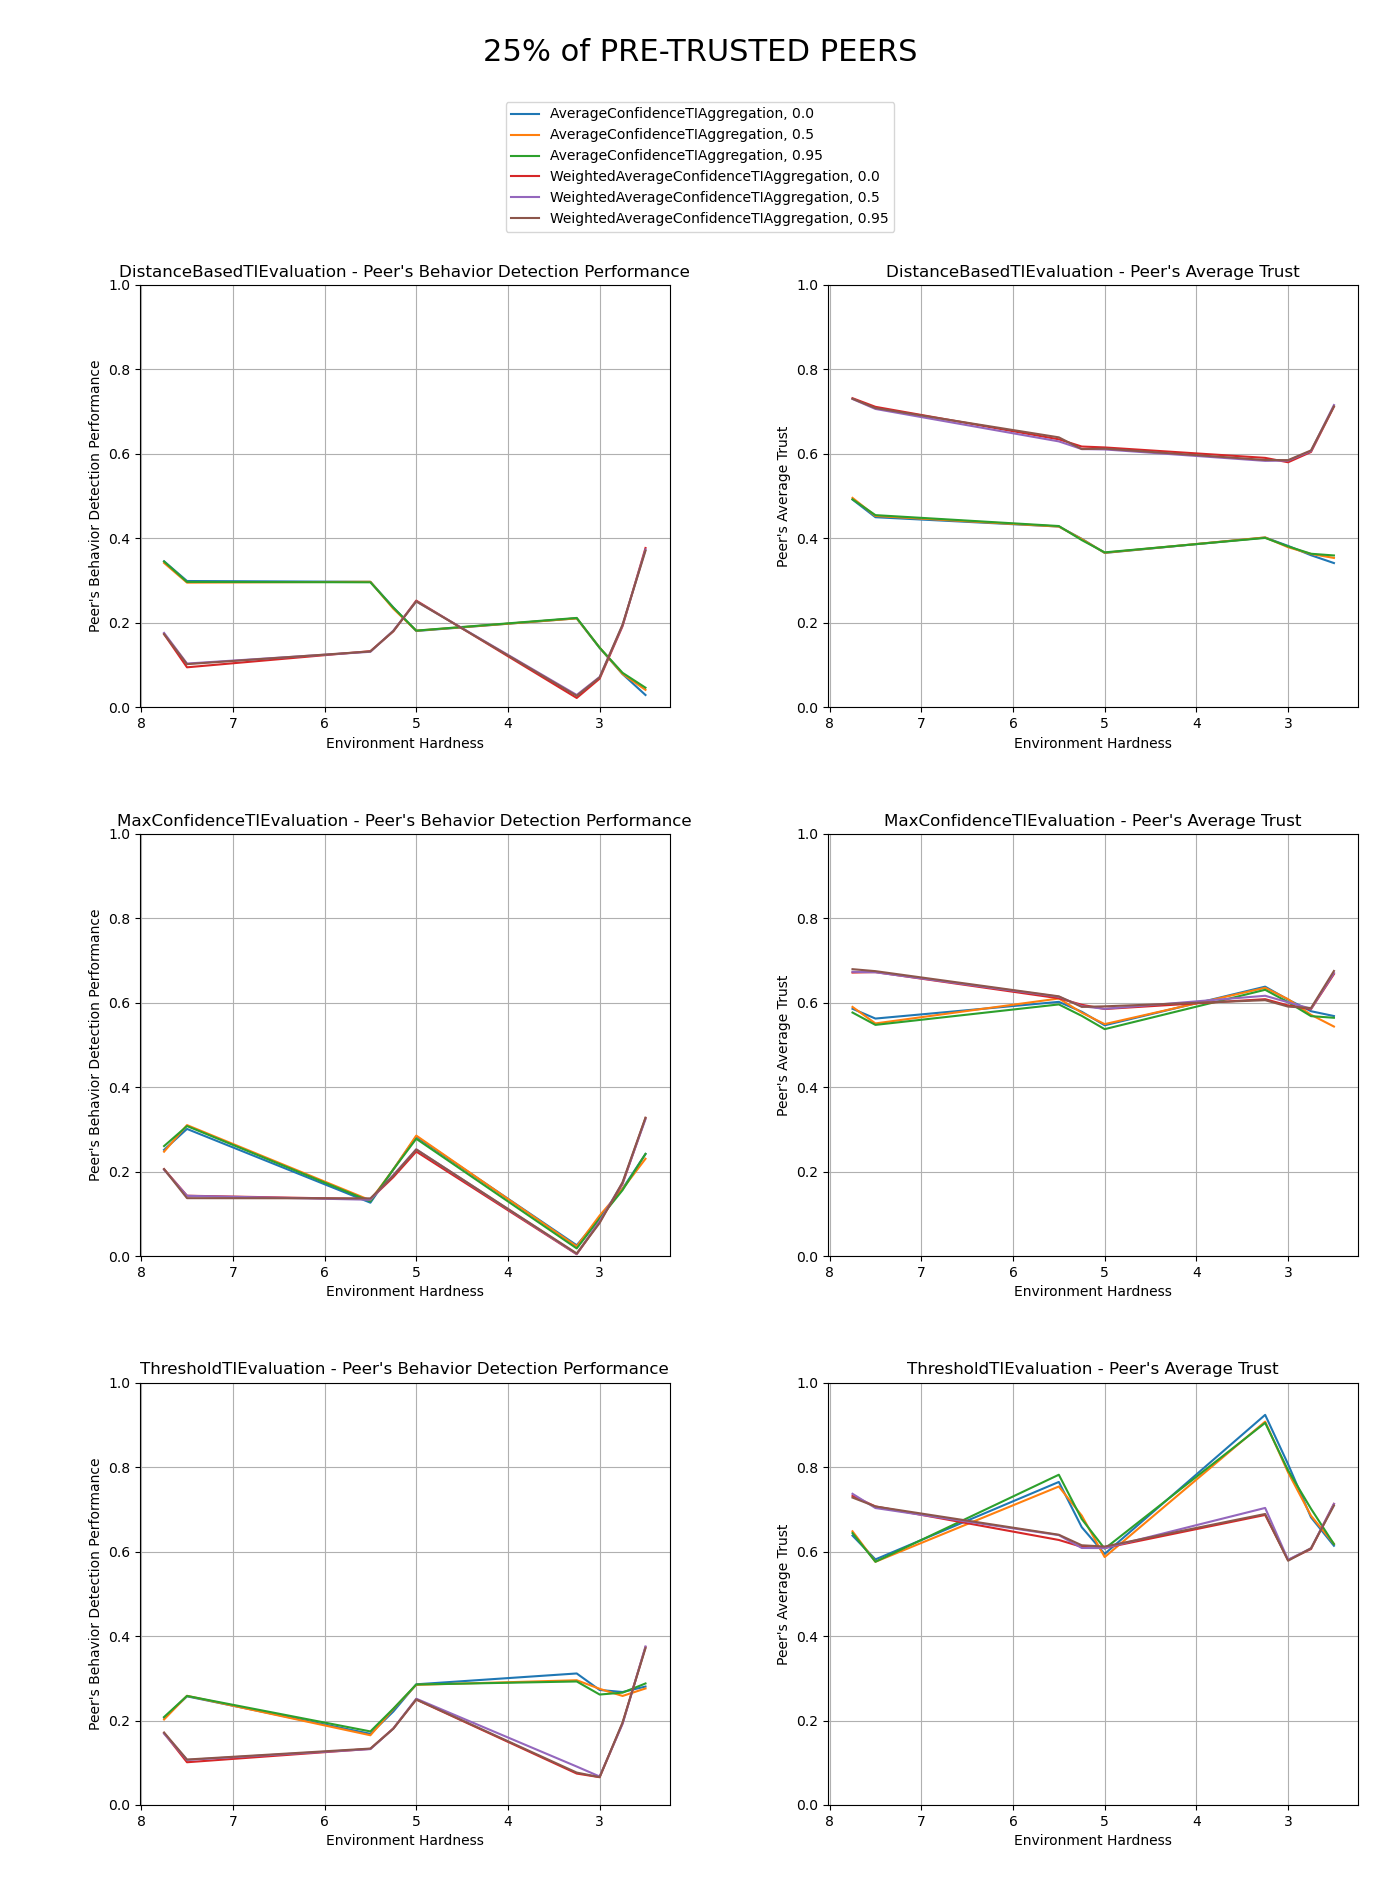
\includegraphics[width=1.0\textwidth]{assets/25_peer_trust.png}
    \caption{Behavior of peer's trust metrics in the different environments for different Fides's setups with \textbf{25\% pre-trusted peers}. On the left side peer's behavior detection performance, on the right side peer's average trust.}
    \label{fig:25-peer-trust}
\end{figure}

Figure~\ref{fig:25-peer-trust}, similarly to Figure~\ref{fig:0-peer-trust} shows the peer's behavior detection performance $pbdp$ on the left side and peer's average trust on the right side.
When we compare Figure~\ref{fig:0-peer-trust} (no pre-trusted peers) with this Figure~\ref{fig:25-peer-trust} (25\% pre-trusted peers), we can clearly see that especially the $pbdp$ metric improved and in all environment it holds that $pbdp \leq 0.4$. 
This means that Fides's ability to identify the true behavior of the peers greatly improved for all interaction evaluation strategies.

The biggest improvement was in strategy $DistanceBasedTIEvaluation$ which had poor performance with no pre-trusted peers in Figure~\ref{fig:0-peer-trust}. However, in the situation with 25\% pre-trusted peers it is now able to detect the true behavior of the peers with the similar precision as the other strategies.
